A Point-Of-Presence (POP) is an artificial demarcation point or interface point between communicating entities.
In our case we are referring to optical fiber interconnection points.
From 2010 until now the guifi.net community has raised six points of presence over the Catalan territory.
This POPs are following the network model of freedom and neutrality specified in the XOLN\ref{XOLN} licence.
Thus anyone is able to connect to them but always respecting the same conditions.
From a general perspective guifi.net community is building a set of neutral exchange points, leaving the
infrastructure available to the individuals, associations or either companies.
\medskip
Figure \ref{fig:fibre_map} shows the fiber network map of guifi.net POPs (not all of them).

\bigskip

The current guifi.net POPs are managed, maintained and also economically sustained for the community. 
To interconnect all of them it is need to use third party infrastructure. The FFTH projects are able to deploy some kilometres
of optical fiber but not hundreds or even thousands.
\newline
In Catalonia there exist a set of deployed fibers which are owned by the Catalan government, available to any entity and 
rented for a regularized price. Most of the guifi.net POPs are connected to such network to interchange data
between them. Figure \ref{fig:xoc_map} shows a slice of the network fiber map provided by the government. 

\begin{figure}[htbp]
  \centering
  \includegraphics[scale=.35]{sect3/figures/pops_network_map.eps} 
%% use convert command to convert formats "convert pops_network_map.png pops_network_map.eps" e.g. 
  \caption{Guifi.net fiber POPs network map}
  \label{fig:fibre_map}
\end{figure}

\begin{figure}[htbp]
  \centering
  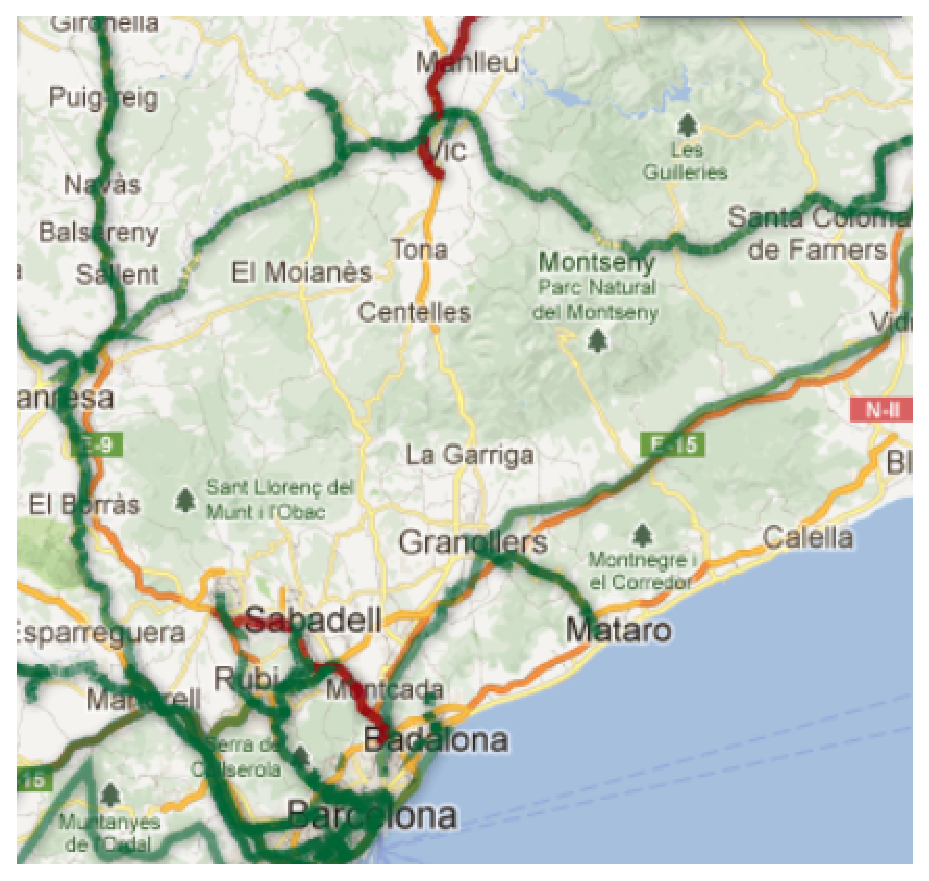
\includegraphics[scale=.5]{sect3/figures/xoc_map.eps} 
  \caption{Available regularized fiber}
  \label{fig:xoc_map}
\end{figure}



\subsection{Pilot's POPs}

\subsubsection{Gurb}

Gurb is a small village in a rural area of the geographical center of Catalonia. Back in 2004 the first guifi.net community
was born here. Probably because of that Gurb is nowadays one of the places where the bottom-up broadband model has more
influence. As seen in section \ref{SECCIO} the community users deployed some optical fiber kilometres to reach the government
infrastructure and connect with other POPs.
\medskip
It is a very important point-of-presence because it allows a small data center provided and maintained by the community.
There are even ISP companies connected to such POP following and using the open-network model to provide Internet
connectivity to end users.


\begin{figure}[htbp]
  \centering
  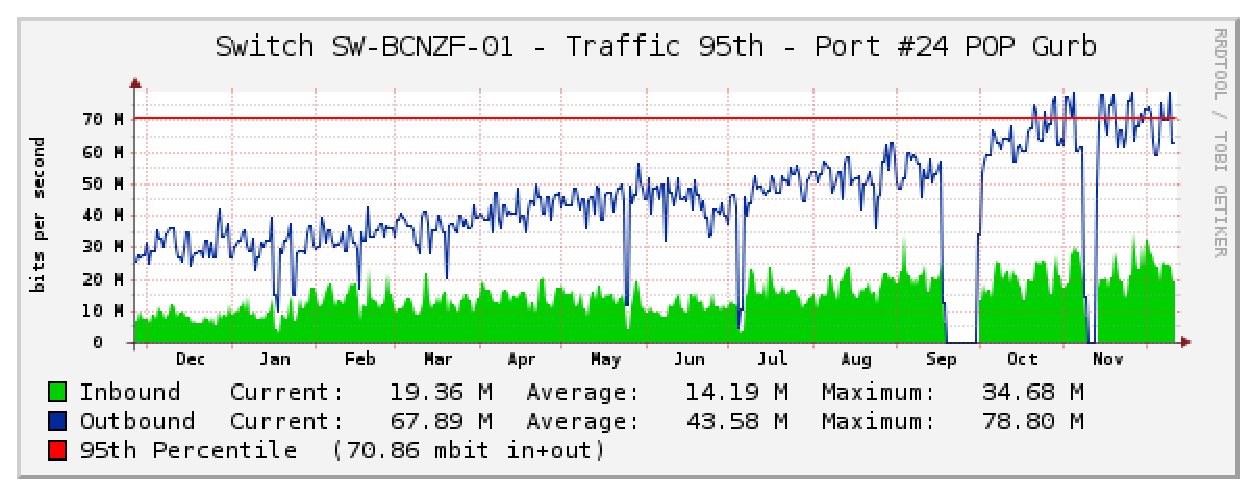
\includegraphics[scale=.65]{sect3/figures/gurb_network_load_year.eps} 
  \caption{Gurb's POP network load (year)}
  \label{fig:gurb_net_load}
\end{figure}


\subsubsection{Vic}

VIC HISTORY ABOUT KIDS AND FORCED WORKD

\begin{figure}[htbp]
  \centering
  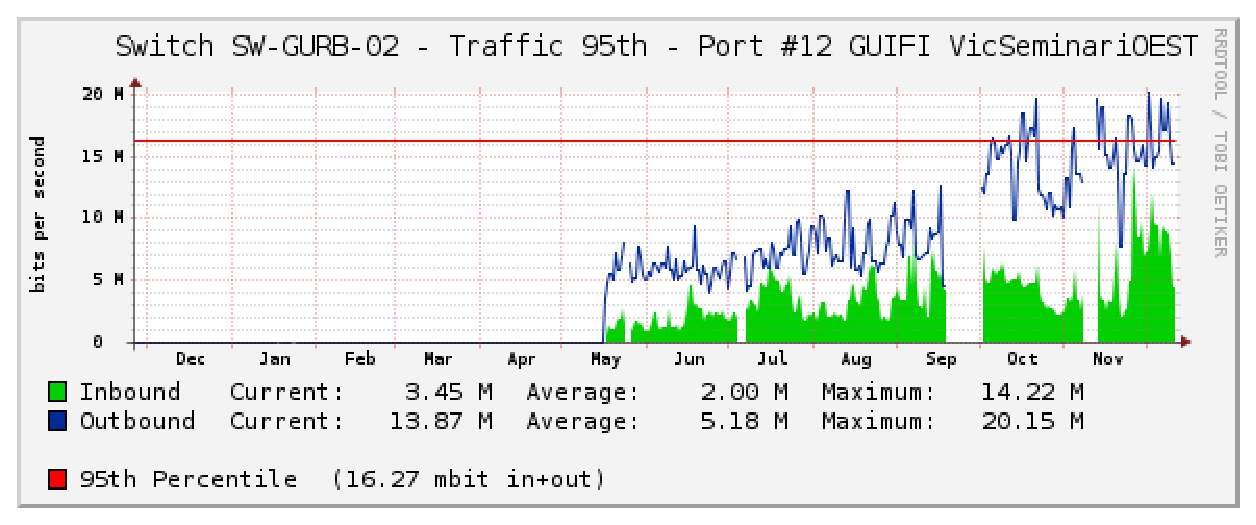
\includegraphics[scale=.65]{sect3/figures/vic_network_load_year.eps} 
  \caption{Vic's POP network load (year)}
  \label{fig:vic_net_load}
\end{figure}



\subsection{Other POPs}

Other points-of-present not directly related with this project are:

\begin{itemize}
	\item Masquefa: blablabla IGLU?

	\item Tortosa: It is a city placed on the sud of Catalonia. The guifi.net users started a goverment's funded project named 
		OpenFPnet\footnote{\url{http://openfpnet.guifi.net}} which tries to create an open and neutral fiber backbone 
		arround the zone and the surrounding villages. Starting from that point they opened a POP to connect with the 
		rest of guifi.net infraestructure. Currently this point-of-presence is economically maintained by some community 
		users grouped in associations and some company with interests of use such fiber.

	\item Barcelona: The Catalonia's capital POP is the one placed in the Internet exchange point CATNIX.
\end{itemize}

\subsubsection{CATNIX}

\bigskip 

CATNIX\footnote{\url{http://www.catnix.net}} is the name of the internet exchange point (IX) of Catalonia. 
It is a physical infrastructure provided by the goberment to leave the network operators exchange their 
information and connect their networks (autonomous systems). 

\medskip
All guifi.net POPs terminate to such infrastructure (as can be shown in figure \ref{fig:fibre_map}) where
all of them connect together to became part of the main community network. 

\medskip
Guifi.net Foundation operates it's own backbone infrastructure using the ASN 49835 (Autonomous System Number). 
An open peering policy is followed to establish peering sessions with all potential partners.
The Foundation is part of the CATNIX, so it is also possible to exchange data with other ISP and
rent Internet uplink directly to an international carrier. Right now there is one symetric Internet gigabit 
available. 
\newline
This is probably the most important POP of the current guifi.net network infraestructure.


\begin{figure}[htbp]
  \centering
  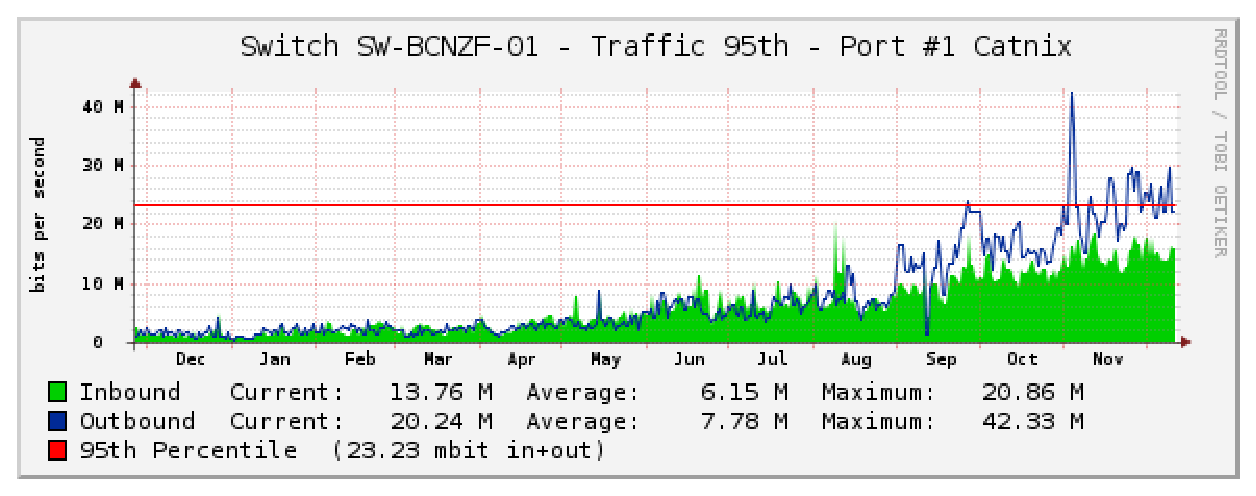
\includegraphics[scale=.65]{sect3/figures/catnix_network_load_year.eps} 
  \caption{CATNIX's POP network load (year)}
  \label{fig:vic_net_load}
\end{figure}


\subsubsection{Tortosa}


\subsubsection{Masquefa}

